% cudaoxide paper -- self-contained skeleton (compiles as-is in an Overleaf-style webapp).
\documentclass[11pt]{article}
\usepackage[margin=1in]{geometry}
\usepackage{amsmath,amssymb}
\usepackage{graphicx}
\usepackage{booktabs}
\usepackage{listings}
\usepackage{tikz}
\usetikzlibrary{arrows.meta,positioning,fit,backgrounds}
\usepackage[numbers,sort&compress]{natbib}
\usepackage{xcolor}
\usepackage[colorlinks=true,allcolors=blue!55!black]{hyperref}
\usepackage{caption}
\captionsetup{font=small,labelfont=bf}
\lstset{basicstyle=\ttfamily\small,breaklines=true,frame=single}

% ===== SHARED HOUSE PREAMBLE (identical to the VLA paper) =====
% Voice: plain, brief, no patronizing analogies, no gushing. Thesis = VIABILITY, never "faster than llama.cpp".

\title{Real FP4 Tensor-Core Code in Pure Rust on a Gaming GPU\\--- with NVIDIA's Own Compiler}
\author{Carter Richardson\\Independent Researcher}
\date{}

\begin{filecontents*}{\jobname.bib}
@misc{cudaoxide, title={cuda-oxide}, howpublished={\url{https://github.com/NVlabs/cuda-oxide}}, note={NVIDIA Labs}}
@misc{llamacpp, title={llama.cpp}, author={Gerganov, Georgi and {the llama.cpp contributors}}, howpublished={\url{https://github.com/ggml-org/llama.cpp}}, year={2023}, note={ggml-org}}
@misc{tinyllama, title={{TinyLlama}: An Open-Source Small Language Model}, author={Zhang, Peiyuan and Zeng, Guangtao and Wang, Tianduo and Lu, Wei}, year={2024}, eprint={2401.02385}, archivePrefix={arXiv}, primaryClass={cs.CL}, howpublished={\url{https://arxiv.org/abs/2401.02385}}}
@misc{ocpmx, title={{OCP} Microscaling Formats ({MX}) Specification, Version 1.0}, author={{Open Compute Project}}, year={2023}, howpublished={\url{https://www.opencompute.org/documents/ocp-microscaling-formats-mx-v1-0-spec-final-pdf}}}
@misc{ptxisa, title={Parallel Thread Execution {ISA}}, author={{NVIDIA}}, howpublished={\url{https://docs.nvidia.com/cuda/parallel-thread-execution/index.html}}, note={\texttt{tcgen05} MMA instructions target \texttt{sm\_100a}/\texttt{sm\_103a}, not \texttt{sm\_120a}}}
@misc{rtx5070ti, title={{GeForce RTX 5070 Ti}}, author={{NVIDIA}}, year={2025}, howpublished={\url{https://blogs.nvidia.com/blog/studio-ai-geforce-rtx-5070-ti-gpu-dlss/}}, note={16\,GB GDDR7, 256-bit, 896\,GB/s}}
@misc{rustcuda, title={The {Rust CUDA} Project}, author={{Rust GPU contributors}}, howpublished={\url{https://github.com/Rust-GPU/Rust-CUDA}}}
@misc{rustgpu, title={Rust {GPU}}, author={{Rust GPU contributors}}, howpublished={\url{https://github.com/Rust-GPU/rust-gpu}}}
@misc{cudarc, title={cudarc: Safe Rust Wrappers for {CUDA}}, author={Lowman, Corey}, howpublished={\url{https://github.com/coreylowman/cudarc}}}
@misc{zluda, title={{ZLUDA}: {CUDA} on Non-{NVIDIA} {GPUs}}, author={Janik, Andrzej}, howpublished={\url{https://github.com/vosen/ZLUDA}}}
@misc{candle, title={candle: Minimalist {ML} Framework for Rust}, author={{Hugging Face}}, howpublished={\url{https://github.com/huggingface/candle}}}
% Commit-pin note: cuda-oxide is pinned to commit 7dbd192 in the repro appendix; the llama.cpp baseline build commit is a fill-at-submission item (built from source vs CUDA 12.9, see App.~A).
\end{filecontents*}

\begin{document}
\maketitle
\begin{abstract}
We report a viability result: an entire Llama-class decoder, written in pure Rust and compiled to PTX by NVIDIA's own experimental first-party Rust$\rightarrow$PTX backend (\texttt{cuda-oxide}), runs FP4-quantized weights on a consumer NVIDIA RTX 5070 Ti and generates coherent English text. On a real TinyLlama-1.1B model quantized to MXFP4, the engine sustains roughly 181 tokens/s of decode throughput at steady state (median over a clean-GPU re-measurement; 188.6\,tok/s in the original session, which the clean run reproduced) --- within about $3.7\times$, or roughly 27\%, of \texttt{llama.cpp}'s decode throughput ($\approx\!664$\,tok/s, Q4\_K\_M, hand-tuned CUDA with CUDA graphs) on the same GPU, on a first, unoptimized cut. Along the way we measured the actual programmable surface of consumer Blackwell (\texttt{sm\_120}) for Rust kernels and found it richer than secondary sources imply: TMA, thread-block clusters with distributed shared memory, and native FP4 block-scaled tensor-core MMA all execute, while the \texttt{tcgen05} 5th-generation tensor-memory MMA pipeline correctly does not. We do \textbf{not} claim supremacy; \texttt{llama.cpp} is faster today, and we say where and why. The contribution is that the path exists end to end --- a coherent LLM, compiled from Rust by NVIDIA's compiler, on a gaming GPU --- and that it lands close on the first attempt, with a clear optimization runway.
\end{abstract}

\section{Introduction}
% Frame samples "coherent, not authoritative" (1.1B greedy).
The claim of this paper is narrow and we keep it narrow: \textbf{viability, not supremacy.}

We took NVIDIA's experimental first-party Rust$\rightarrow$PTX compiler, \texttt{cuda-oxide} (alpha), and used it to write every kernel of a Llama-class decoder in pure Rust --- RMSNorm, RoPE, grouped-query flash decode, SwiGLU, and FP4-quantized matrix--vector projections --- with no hand-written CUDA C++ in the inference path. We compiled those kernels to PTX through NVIDIA's backend, loaded a real TinyLlama-1.1B model~\citep{tinyllama} quantized to 4-bit MXFP4, and generated text on a consumer RTX 5070 Ti.

The headline artifact is a single generation. Given the prompt \emph{``The main advantage of running a neural network on a GPU instead of a CPU is''}, the engine continued:

\begin{quote}\itshape
\ldots that it can handle larger datasets and faster processing speeds. This means that the model can learn more complex patterns and make more accurate predictions, which can lead to better results in real-world applications.
\end{quote}

That is grammatical, on-topic, greedy-decoded text from a 4-bit-quantized LLM, produced entirely through NVIDIA's Rust$\rightarrow$PTX backend on a gaming GPU. It is 1.1B-parameter greedy output --- coherent, not authoritative; we use it to demonstrate that the forward pass is numerically correct end to end, not as a source of fact.

\textbf{Contributions.}
\begin{enumerate}
\item A \textbf{measured capability map} of consumer Blackwell (\texttt{sm\_120}, RTX 5070 Ti) for Rust GPU kernels (\S\ref{sec:cap}), correcting two ``datacenter-only'' assumptions from our pre-build research --- one echoing a community Blackwell wiki, one our own conservative read --- that measurement refutes (TMA and clusters/DSMEM both work), while confirming the expected datacenter exclusions (\texttt{tcgen05}/TMEM, WGMMA, CTA-pair multicast).
\item A pinned, CPU-reference-validated \textbf{FP4 (NVFP4/MXFP4) \texttt{m16n8k64} block-scaled tensor-core MMA} driven from pure Rust through \texttt{cuda-oxide} (\S\ref{sec:fp4}) --- the full element and scale-factor operand layout, which, to the best of the positioning in \S\ref{sec:related}, is the first pure-Rust FP4 tensor-core MMA demonstrated on consumer Blackwell (we did not perform an exhaustive prior-art search; see the hedge in \S\ref{sec:fp4}).
\item A complete \textbf{pure-Rust FP4 decode engine} (\S\ref{sec:e2e}): per-kernel CPU-parity validation, an end-to-end forward pass on real weights, and coherent text from a real model.
\item An \textbf{honest head-to-head} against \texttt{llama.cpp}~\citep{llamacpp} on the same GPU and model (\S\ref{sec:e2e}), where we lose on raw decode speed by about $3.7\times$, with a gap analysis that attributes the difference to specific, addressable engineering --- not to the language or the compiler.
\end{enumerate}

We are deliberate about framing throughout. Every speed claim carries its measurement and configuration; every novelty claim is hedged; and where a weak signal corroborates a strong conclusion, the two are stated as separate sentences with separate weight, never fused.

\section{Background: cuda-oxide and consumer Blackwell}
\texttt{cuda-oxide}~\citep{cudaoxide} is NVIDIA's experimental, alpha-stage compiler backend that lowers Rust (via a custom \texttt{rustc} codegen backend over LLVM) directly to PTX, NVIDIA's virtual ISA, which \texttt{ptxas} then assembles to SASS for a specific GPU. The toolchain ships device intrinsics for the modern PTX feature set, a \texttt{cargo oxide} driver, and a set of example kernels. It is pre-1.0 and moves quickly; the results here are pinned to a specific commit (\S\ref{sec:repro}) and should be treated as a snapshot. The significance for this work is that the kernel source is ordinary \texttt{no\_std} Rust --- the same language as the host harness, with shared \texttt{\#[repr(C)]} data layouts --- rather than CUDA C++ with a Rust shim. The inference path contains no hand-written CUDA C++.

The RTX 5070 Ti is a GB203 part with compute capability 12.0 (\texttt{sm\_120}). It is a Blackwell-generation consumer GPU, distinct from datacenter Blackwell (\texttt{sm\_100}, e.g.\ B200). The two share the Blackwell numeric formats but differ in the tensor-core pipeline: datacenter Blackwell adds the 5th-generation tensor-memory (\texttt{tcgen05}/TMEM) MMA path and its associated speed-of-light GEMM, which consumer Blackwell does not have. A central question for any Rust-on-Blackwell effort is exactly \emph{which} of the advertised Blackwell features are reachable on the consumer part; \S\ref{sec:cap} answers it by measurement.

Blackwell tensor cores support 4-bit floating-point operands in the E2M1 format (1 sign, 2 exponent, 1 mantissa bit) with block-wise scale factors. \textbf{MXFP4}~\citep{ocpmx} uses 32-element blocks with a power-of-two (\texttt{ue8m0}) scale per block; \textbf{NVFP4}~\citep{ptxisa} uses 16-element blocks with a fractional (\texttt{ue4m3}) scale per block. Both are weight-only quantization targets here: the model's projection weights are stored in FP4 with per-block scales, while activations remain higher precision. FP4 roughly quarters weight traffic relative to f16, which is the lever that matters for bandwidth-bound decode (\S\ref{sec:e2e}).

\section{Related Work}
\label{sec:related}
\textbf{Rust on GPUs.} Several toolchains compile Rust toward GPU targets: \texttt{rust-gpu}~\citep{rustgpu} (SPIR-V/Vulkan), the Rust-CUDA project's \texttt{rustc\_codegen\_nvvm}~\citep{rustcuda} (Rust$\rightarrow$NVVM$\rightarrow$PTX), and host-side binding and launch crates such as \texttt{cudarc}~\citep{cudarc}; \texttt{ZLUDA}~\citep{zluda} re-targets CUDA binaries onto non-NVIDIA hardware. \texttt{cuda-oxide} differs in being NVIDIA's own first-party experimental Rust$\rightarrow$PTX backend, which is the toolchain whose consumer-Blackwell surface we measure.

\textbf{FP4 / MXFP4 inference.} Block-scaled 4-bit floating point --- MXFP4 under the OCP microscaling specification~\citep{ocpmx} and NVFP4 in NVIDIA's Blackwell tensor-core ISA~\citep{ptxisa} --- is documented at the format and hardware level, but production FP4 kernels today are predominantly CUDA C++/PTX. We are not aware of a pure-Rust driver of the \texttt{m16n8k64} block-scaled FP4 MMA, which is the operand-layout contribution of \S\ref{sec:fp4}.

\textbf{Rust LLM inference engines.} Rust inference stacks such as \texttt{candle}~\citep{candle} run model forward passes from Rust but dispatch GPU compute through vendor kernels or CUDA C++ rather than compiling their kernels from Rust; \texttt{llama.cpp}~\citep{llamacpp} is our hand-tuned CUDA baseline (\S\ref{sec:e2e}). The gap we fill is an end-to-end decoder whose every kernel is compiled from Rust by NVIDIA's backend.

\section{What executes on consumer sm\_120 (and what correctly rejects)}
\label{sec:cap}
% Corroborating & weaker = LLVM CannotYetSelect at sm_120a. cuda-oxide DOES implement tcgen05 -- never "codegen path absent".
Before building an engine we measured what actually runs. We compiled and executed a curated set of the backend's own example kernels on the real 5070 Ti and classified each by its runtime log marker --- a kernel counts as executing only if it emits an explicit correctness marker, with datacenter-target rejects and self-skips caught first. (The classifier was tightened after review so that it no longer matches PTX-generation boilerplate; it requires a genuine execution-success marker.) Table~\ref{tab:cap} summarizes the surface.

\begin{table}[t]\centering
\begin{tabular}{lll}
\toprule
feature & sm\_120 result & evidence\\
\midrule
atomics / sharedmem / warp-reduce / GEMM & executes & per-example PASS\\
TMA copy + pipeline & executes & 4096/4096 match\\
clusters + DSMEM & executes & cross-block reduction PASSED\\
tcgen05 / tcgen05\_matmul / gemm\_sol & rejects & driver INVALID\_PTX / requires sm\_100\\
WGMMA & rejects & Hopper-only\\
TMA multicast & rejects & sm\_100a\\
\bottomrule
\end{tabular}
\caption{Consumer Blackwell capability surface for Rust kernels, measured on an RTX 5070 Ti via \texttt{cuda-oxide} examples. TMA and clusters with distributed shared memory both execute as shipped examples here, and FP4 block-scaled tensor-core MMA is validated directly in \S\ref{sec:fp4} (no shipped example exercises it). Note that the CUDA-core GEMM examples emit FMA, not tensor-core MMA.}
\label{tab:cap}
\end{table}

\textbf{On the GEMM rows and tensor-core reachability.} The shipped \texttt{gemm} and \texttt{tiled\_gemm} examples computed correctly (2630 and 3530\,GFLOPS, max relative error \texttt{1.5e-5}), but their PTX contains no \texttt{mma}/\texttt{wgmma}: these are CUDA-core FMA figures, not tensor-core peak, and we report them as such. The tensor cores themselves are reachable --- a hand-written \texttt{mma.sync} assembles under \texttt{ptxas -arch=sm\_120a} (cubin emitted), and \S\ref{sec:fp4} drives the FP4 block-scaled variant with real operands --- but no shipped example exercises them, which is why we validate that path directly in isolation rather than inferring it from a stock benchmark.

\textbf{On the \texttt{tcgen05} rejection, two separate facts, kept separate.} These corroborate each other but carry different weight, and we do not fuse them. The load-bearing fact is hardware: on a real \texttt{sm\_120} part the CUDA driver returns \texttt{INVALID\_PTX} when loading a \texttt{tcgen05} module, because consumer Blackwell lacks the 5th-generation tensor-memory (\texttt{tcgen05}/TMEM) MMA path that datacenter \texttt{sm\_100} adds~\citep{ptxisa}. That is \emph{why} the feature does not run, and it is the claim. The corroborating, weaker, separate fact is toolchain: \texttt{cuda-oxide} \emph{does} implement the \texttt{tcgen05} intrinsics and emits real \texttt{tcgen05.*} PTX (its codegen table even optimistically lists \texttt{sm\_120}/\texttt{sm\_120a}), and when \emph{forced} to the \texttt{sm\_120a} target the backend hits an LLVM \texttt{CannotYetSelect} on the instruction sequence --- an instruction-selection gap at that target. A reviewer can open the backend source and see the codegen path present, so this is corroboration only. \textbf{We never claim the codegen path is absent}; the hardware reject is the conclusion, and the selection gap is a footnote to it.

\textbf{The headline finding.} The common shorthand ``consumer Blackwell is just a cut-down datacenter Blackwell'' is wrong in both directions. Consumer \texttt{sm\_120} \emph{does} run TMA, thread-block clusters with distributed shared memory, and native FP4 block-scaled tensor-core MMA --- features frequently assumed datacenter-only --- in one case contradicting a community Blackwell wiki's ``cluster size 1'' claim, in the other overturning our own conservative pre-build assessment that TMA was probably unusable on the 5070 Ti. Our own pre-build research correctly nailed the consumer/datacenter \texttt{tcgen05}/TMEM split but inherited two ``datacenter-only'' claims that measurement refutes: that TMA does not work usefully on the 5070 Ti (it does --- \texttt{cp.async.bulk.tensor} and a TMA pipeline both run correctly), and that clusters are limited to size 1 (a $4\times1\times1$ cluster performing a cross-block DSMEM reduction passes). Consumer \texttt{sm\_120} \emph{does not} run the \texttt{tcgen05}/TMEM MMA pipeline, its speed-of-light GEMM, WGMMA, or CTA-pair TMA multicast --- those are datacenter \texttt{sm\_100a} or Hopper. So the programmable surface for Rust kernels on consumer Blackwell is full \texttt{mma.sync} tensor cores including FP4, TMA, clusters/DSMEM, \texttt{cp.async}, scoped atomics, \texttt{bf16x2}, and dp4a --- everything except the \texttt{tcgen05}/TMEM datacenter MMA path. That surface is the substrate the engine in \S\ref{sec:e2e} is built on.

\section{FP4 block-scaled MMA (m16n8k64) in Rust}
\label{sec:fp4}
% From trackb/FP4_M16N8K64_LAYOUT.md -- pinned, validated 0 mismatches. Good TikZ figure candidate (fragment/scale layout).
The FP4 block-scaled MMA is the operand-layout-heavy part of the work, so we validated it in isolation before wiring it into the engine. The MXFP4 path uses, at the PTX level:

\begin{lstlisting}
mma.sync.aligned.m16n8k64.row.col.kind::mxf4.block_scale.scale_vec::2X.f32.e2m1.e2m1.f32.ue8m0
  {d0,d1,d2,d3}, {a0,a1,a2,a3}, {b0,b1}, {c0,c1,c2,c3},
  sa, {byte_id,thread_id}, sb, {byte_id,thread_id};
\end{lstlisting}

(NVFP4 uses \texttt{kind::mxf4nvf4}, \texttt{scale\_vec::4X}, \texttt{.ue4m3}.) The operand fragments are A $= 4\times$\texttt{.b32}, B $= 2\times$\texttt{.b32}, C/D $= 4\times$\texttt{.f32}, with 4-bit E2M1 values packed 8 per \texttt{.b32}. The scale operands \texttt{sa}/\texttt{sb} are \texttt{.b32} registers; the accompanying byte-id/thread-id are \emph{immediate integer constants}, not registers --- supplying them as registers was the source of an early \texttt{ptxas} parse error.

\textbf{Target gate.} The block-scaled MMA requires \texttt{.target sm\_120a} (the architecture-\emph{specific} variant). Plain \texttt{sm\_120} rejects it with \emph{``Instruction `mma with block scale' not supported on .target `sm\_120'.''} For \texttt{nvcc} this means \texttt{-gencode arch=compute\_120a,code=sm\_120a}; for \texttt{cuda-oxide}, build with \texttt{--arch sm\_120a}.

\textbf{Numerical validation.} We validated correctness against a CPU reference at three levels, all with zero mismatches. An all-ones test (A $=$ B $= 1.0$, scale $= 1.0$) yields every output element $= \sum_{k=0}^{63} 1\cdot 1 = 64.0$; measured 128/128 $= 64.0$. This proves the instruction executes, the E2M1 encoding and \texttt{ue8m0} scale decode correctly, and the $k=64$ accumulation is right, without depending on the exact per-thread fragment mapping. The element fragment mapping was then pinned against non-uniform FP4 data with full CPU-reference parity (0/128 mismatch), recording the exact \texttt{m16n8k64} E2M1 thread/register layout. The scale-factor layout was pinned with non-uniform power-of-two scales (0/128 mismatch): \texttt{scale\_vec::2X}, $K=64\rightarrow 2$ blocks/row, \texttt{ue8m0} byte $= 127 + \log_2(\text{scale})$. With this, a full FP4 GEMM with per-block scales is buildable.

\textbf{The pinned layout.} Table~\ref{tab:fp4layout} records the recovered \texttt{m16n8k64} thread/register map. Writing $g=\lfloor\text{lane}/4\rfloor$ ($0\ldots7$) and $t=\text{lane}\bmod 4$ ($0\ldots3$), with the low nibble of each \texttt{.b32} holding the lowest $K$ index and eight E2M1 values packed per register, the element positions are as shown in Table~\ref{tab:fp4layout} and Figure~\ref{fig:fp4layout}; the E2M1 magnitudes are $\{0,0.5,1,1.5,2,3,4,6\}$ for code bits $0\ldots2$ with bit~3 the sign ($1.0=\texttt{0x2}$). For the scale factors, \texttt{scale\_vec::2X} with $K=64$ gives two 32-element blocks per row, so each \texttt{.b32} scale register holds four \texttt{ue8m0} bytes: $\texttt{sa}=[\,\text{SFA}[g][0],\text{SFA}[g][1],\text{SFA}[g{+}8][0],\text{SFA}[g{+}8][1]\,]$ and $\texttt{sb}=[\,\text{SFB}[0][g],\text{SFB}[1][g],\ldots\,]$ in its low two bytes (replicated to the high two). All four threads of a quad carry the same \texttt{sa}/\texttt{sb}; the hardware selects within them via the \texttt{\{0,0\}} byte-id/thread-id immediates, and the \texttt{ue8m0} byte encodes the power-of-two scale as $127+\log_2(\text{scale})$ ($1.0=\texttt{0x7f}$). Pinning this exact layout is what turns a single validated MMA into a buildable per-block-scaled GEMM, and it is the part a re-implementation would otherwise have to rediscover by trial against \texttt{ptxas}.

\begin{figure}[t]\centering
\resizebox{\textwidth}{!}{%
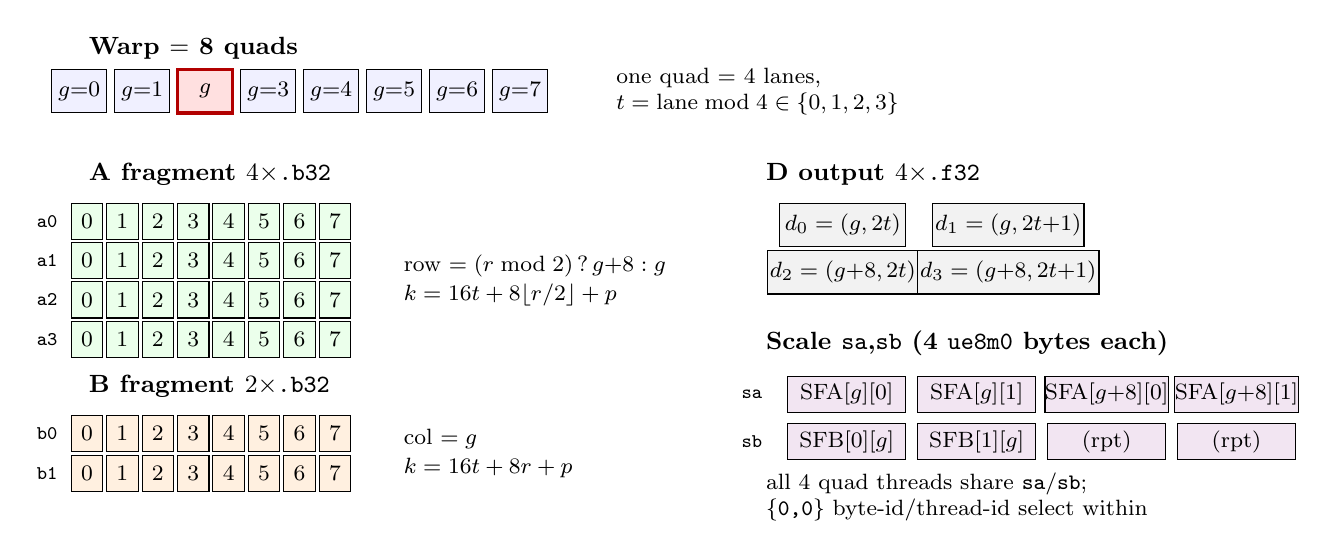
\begin{tikzpicture}[
  font=\footnotesize,
  quad/.style={draw, minimum width=7mm, minimum height=5.5mm, inner sep=1pt},
  nib/.style={draw, minimum width=4mm, minimum height=4.6mm, inner sep=0pt},
  rl/.style={font=\scriptsize\ttfamily},
  pan/.style={font=\small\bfseries}
]
% Panel A: warp -> 8 quads
\node[pan, anchor=west] at (0,0.55) {Warp $=$ 8 quads};
\foreach \g in {0,...,7} {\node[quad, fill=blue!6] at (\g*0.8,0) {$g{=}\g$};}
\node[quad, draw=red!70!black, very thick, fill=red!12] at (1.6,0) {$g$};
\node[anchor=west, align=left] at (6.7,0) {one quad $=$ 4 lanes,\\ $t=\text{lane}\bmod4\in\{0,1,2,3\}$};
% Panel B: A fragment
\node[pan, anchor=west] at (0,-1.05) {A fragment $4\times$\texttt{.b32}};
\foreach \r/\y in {0/-1.65,1/-2.15,2/-2.65,3/-3.15} {
  \node[rl, anchor=east] at (-0.15,\y) {a\r};
  \foreach \p in {0,...,7} {\node[nib, fill=green!8] at (\p*0.45+0.1,\y) {$\p$};}
}
\node[anchor=west, align=left] at (4.0,-2.4) {row $=(r\bmod2)\,?\,g{+}8:g$\\[1pt] $k=16t+8\lfloor r/2\rfloor+p$};
% Panel C: B fragment
\node[pan, anchor=west] at (0,-3.75) {B fragment $2\times$\texttt{.b32}};
\foreach \r/\y in {0/-4.35,1/-4.85} {
  \node[rl, anchor=east] at (-0.15,\y) {b\r};
  \foreach \p in {0,...,7} {\node[nib, fill=orange!12] at (\p*0.45+0.1,\y) {$\p$};}
}
\node[anchor=west, align=left] at (4.0,-4.6) {col $=g$\\[1pt] $k=16t+8r+p$};
% Panel D: D output positions
\node[pan, anchor=west] at (8.6,-1.05) {D output $4\times$\texttt{.f32}};
\node[quad, minimum width=16mm, fill=gray!10] at (9.7,-1.7) {$d_0=(g,2t)$};
\node[quad, minimum width=16mm, fill=gray!10] at (11.8,-1.7) {$d_1=(g,2t{+}1)$};
\node[quad, minimum width=16mm, fill=gray!10] at (9.7,-2.3) {$d_2=(g{+}8,2t)$};
\node[quad, minimum width=16mm, fill=gray!10] at (11.8,-2.3) {$d_3=(g{+}8,2t{+}1)$};
% Panel E: scale registers
\node[pan, anchor=west] at (8.6,-3.2) {Scale \texttt{sa},\texttt{sb} (4 \texttt{ue8m0} bytes each)};
\node[rl, anchor=east] at (8.8,-3.85) {sa};
\node[nib, minimum width=15mm, fill=violet!10] at (9.75,-3.85) {SFA$[g][0]$};
\node[nib, minimum width=15mm, fill=violet!10] at (11.4,-3.85) {SFA$[g][1]$};
\node[nib, minimum width=15mm, fill=violet!10] at (13.05,-3.85) {SFA$[g{+}8][0]$};
\node[nib, minimum width=15mm, fill=violet!10] at (14.7,-3.85) {SFA$[g{+}8][1]$};
\node[rl, anchor=east] at (8.8,-4.45) {sb};
\node[nib, minimum width=15mm, fill=violet!10] at (9.75,-4.45) {SFB$[0][g]$};
\node[nib, minimum width=15mm, fill=violet!10] at (11.4,-4.45) {SFB$[1][g]$};
\node[nib, minimum width=15mm, fill=violet!10] at (13.05,-4.45) {(rpt)};
\node[nib, minimum width=15mm, fill=violet!10] at (14.7,-4.45) {(rpt)};
\node[anchor=west, align=left] at (8.6,-5.15) {all 4 quad threads share \texttt{sa}/\texttt{sb};\\ \texttt{\{0,0\}} byte-id/thread-id select within};
\end{tikzpicture}%
}
\caption{Single-quad fragment map for the \texttt{m16n8k64} block-scaled FP4 MMA, drawn from the validated layout of Table~\ref{tab:fp4layout}. A warp's 32 lanes split into 8 quads indexed $g=\lfloor\text{lane}/4\rfloor$, each holding 4 lanes $t=\text{lane}\bmod4$; one quad (highlighted) is expanded. Each \texttt{.b32} register packs eight E2M1 values at nibble positions $p=0\ldots7$ (low nibble $=$ lowest $K$), and $r$ is the register index within a fragment. The A fragment ($a_0\ldots a_3$) and B fragment ($b_0,b_1$) give each value's matrix row/column and $K$ index; the D fragment ($d_0\ldots d_3$) gives the four output positions. All four threads of the quad carry the same scale registers \texttt{sa}/\texttt{sb} (four \texttt{ue8m0} bytes each, \texttt{ue8m0} byte $=127+\log_2(\text{scale})$); the \texttt{\{0,0\}} byte-id/thread-id immediates select within them.}
\label{fig:fp4layout}
\end{figure}

\begin{table}[t]\centering
\begin{tabular}{lll}
\toprule
operand & fragment & element position (nibble $p=0\ldots7$, register index $r$)\\
\midrule
A & $16\times64$ row-major, $a_0\ldots a_3$ & row $=(r\bmod2)\,?\,g{+}8:g$, \quad $k=16t+8\lfloor r/2\rfloor+p$\\
B & $64\times8$ col-major, $b_0,b_1$ & col $=g$, \quad $k=16t+8r+p$\\
D & $16\times8$, $d_0\ldots d_3$ & $(g,2t),\,(g,2t{+}1),\,(g{+}8,2t),\,(g{+}8,2t{+}1)$\\
\bottomrule
\end{tabular}
\caption{Pinned \texttt{m16n8k64} E2M1 operand layout, recovered against a CPU reference (0/128 mismatch). Lane decomposes as $g=\lfloor\text{lane}/4\rfloor$, $t=\text{lane}\bmod4$; each \texttt{.b32} packs eight E2M1 values, low nibble the lowest $K$.}
\label{tab:fp4layout}
\end{table}

\textbf{Driven from pure Rust.} The MMA runs through \texttt{cuda-oxide}, not only through \texttt{nvcc}: the \texttt{fp4\_mma} example produces $\checkmark$ all 128 $= 64.0$. Because the backend's inline-asm macro allows only a single \texttt{out} operand, the MMA plus its four \texttt{st.global} stores live in one memory-clobbering inline-asm block writing through a per-lane pointer.

\textbf{Novelty hedge.} To the best of the positioning in \S\ref{sec:related}, this is the first pure-Rust FP4 tensor-core MMA demonstrated on consumer Blackwell. We did \emph{not} perform an exhaustive prior-art search, so we state this as a belief, not an established first.

\section{End-to-end: TinyLlama-1.1B MXFP4 decode}
\label{sec:e2e}

\textbf{Kernels, each CPU-parity validated.} Every kernel in the forward pass was built in pure Rust and gated against a CPU reference before assembly (Table~\ref{tab:kernels}). Reusable patterns: block-reduce via warp shuffle plus shared-memory partials (RMSNorm, softmax); a precomputed rotary cos/sin cache passed in from the host (no device transcendentals on the hot path); device \texttt{libdevice} math where needed.

\begin{table}[t]\centering
\begin{tabular}{llll}
\toprule
kernel & example & dims & result (max rel.\ err)\\
\midrule
RMSNorm & \texttt{llama\_rmsnorm} & dim 2048 & 7e-7, 0/2048\\
RoPE (rotate-half, HF) & \texttt{llama\_rope} & 32 heads $\times$ 64, $\theta{=}5\mathrm{e}5$ & 1.4e-5, 0/2048\\
Flash-attn decode (GQA) & \texttt{llama\_attn\_decode} & 32 q / 8 kv heads, seq 512 & 4.4e-5, 0/2048\\
FP4 decode GEMV & \texttt{fp4\_gemv} & up to 16384$\times$4096 & $\sim$1.3e-3, 0 bad\\
\bottomrule
\end{tabular}
\caption{Per-kernel CPU-parity validation. Every forward-pass kernel was gated against a CPU reference before assembly.}
\label{tab:kernels}
\end{table}

\textbf{End-to-end assembly.} The full forward pass runs with FP4 weights on every projection: RMSNorm $\rightarrow$ FP4 QKV $\rightarrow$ RoPE $\rightarrow$ GQA flash-decode $\rightarrow$ FP4 output projection $\rightarrow$ residual $\rightarrow$ RMSNorm $\rightarrow$ FP4 SwiGLU MLP $\rightarrow$ residual, repeated across layers, then a final norm and FP4 LM head (vocab 128{,}256), with a KV cache. On a Llama-1B configuration (ctx 512, 32 tokens timed, random weights) it sustains 4.51\,ms/token $= 221.6$\,tokens/s, producing finite logits and a valid argmax. This is a \emph{pipeline-performance} number on random weights --- the token IDs are meaningless; output quality is established separately below.

\textbf{The bandwidth-bound-decode thesis.} Single-token decode is dominated by streaming the model's weights once per token, not by arithmetic. At a 896\,GB/s memory ceiling on the 5070 Ti~\citep{rtx5070ti}, the relevant metric for the FP4 GEMV (which carries the QKV, output, MLP, and LM-head projections) is the fraction of that ceiling it reaches. This is \emph{why} the missing \texttt{tcgen05} datacenter MMA path barely hurts decode: decode does not need speed-of-light GEMM, it needs bandwidth. Figure~\ref{fig:bw} reports measured FP4 GEMV weight-streaming bandwidth. Three measured lessons, stated as measured rather than assumed: a \texttt{const [f32;8]} decode LUT lowers to local memory under this backend, so decoding E2M1 arithmetically is faster; the backend did \emph{not} vectorize a \texttt{repr(C)} $4\times$\texttt{u32} struct load to \texttt{ld.global.v4} (it stayed scalar \texttt{b32}), and fewer-larger iterations \emph{hurt} throughput by reducing memory-level parallelism, so the 16-iteration \texttt{u32} stream beat the 4-iteration 128-bit version; and staging the activation vector in shared memory once per block removes the $N\times$ re-read. The climb from 30\% to 41\% with size indicates the small-matrix figure is a launch/occupancy ramp, not kernel inefficiency. Notably, three of the capability surprises of \S\ref{sec:cap} --- TMA, \texttt{cp.async}, and clusters with distributed shared memory --- are exactly the weight-streaming levers this kernel does \emph{not} yet use: it streams with plain scalar \texttt{ld.global} and stages activations in ordinary shared memory. Async-copy (\texttt{cp.async}/TMA) pipelining, hand-vectorized shared-memory loads (the backend would not emit \texttt{ld.global.v4} on its own), and multi-row-per-warp scheduling are the named, measured-as-available levers toward peak, left to dedicated perf work.

\begin{figure}[t]\centering
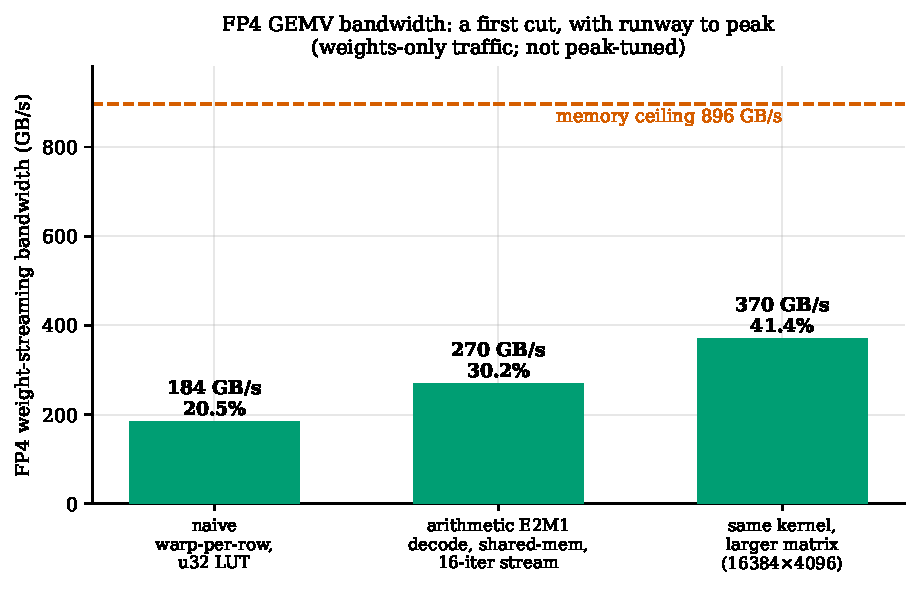
\includegraphics[width=0.92\linewidth]{figs/fig_bandwidth.pdf}
\caption{FP4 GEMV weight-streaming bandwidth (weights-only, the FP4-shrunk traffic), a first cut, not peak-tuned: from a naive \texttt{u32}-LUT kernel ($\sim$184\,GB/s, 20.5\% of the 896\,GB/s ceiling), to arithmetic E2M1 decode with a shared-memory activation stream (270\,GB/s, 30.2\%), to 41.4\% on a larger matrix. The climb with size indicates a launch/occupancy ramp, not kernel inefficiency.}
\label{fig:bw}
\end{figure}

\textbf{A real model: coherent text from TinyLlama-1.1B.} The engine loads the real TinyLlama-1.1B safetensors~\citep{tinyllama} (bf16 $\rightarrow$ f32 on parse), quantizes every projection to MXFP4 (E2M1 with a per-32 absmax f32 scale) on the host, and performs embedding lookup, prefill, and greedy generation with device argmax (no per-token logit copy to the host). Tokenization (encode/decode) is a standalone Hugging Face \texttt{tokenizers} \texttt{cargo} binary kept out of the \texttt{cuda-oxide} build, so the compiled inference path stays purely the kernels. The prompt quoted in \S1 produced the continuation shown there, and other prompts in the same domain give similarly coherent output. Model load and host quantization take $\sim$22\,s; generation runs at 188.6\,tokens/s in the original session, reproduced on a clean GPU at steady state (below). This establishes what the random-weight run could not: safetensors load is correct, MXFP4 weight-only quantization preserves output quality, the full forward pass is correct on real weights, and end-to-end generation works.

\textbf{Head-to-head with \texttt{llama.cpp}.} We compared against \texttt{llama.cpp}~\citep{llamacpp} on the same GPU and the same model, both at 4-bit. \texttt{llama.cpp} was built from source against the full CUDA 12.9 toolkit (the 13.1 toolkit on this machine lacks cuBLAS; 12.9 is the full one and its \texttt{ptxas} supports \texttt{sm\_120a}), with \texttt{CMAKE\_CUDA\_ARCHITECTURES=120}, and measured with \texttt{llama-bench} on TinyLlama-1.1B Q4\_K\_M, all layers on GPU. To avoid single-run artifacts, we re-measured both engines on an \emph{uncontended} GPU in the same session, at steady state --- timing 200 generated tokens, enough to clear the GPU's post-idle clock-ramp. Ours held a tight 176--193\,tok/s (median 181 over five runs) and \texttt{llama.cpp} 634--664\,tok/s ($\approx\!664$), reproducing the original-session figures of 188.6 and 633.9. We report the reproducible clean-GPU medians: \textbf{ours $\approx 181$ vs \texttt{llama.cpp} $\approx 664$ --- roughly $3.7\times$, about 27\% of its decode throughput} (Figure~\ref{fig:h2h}). A short timing window, by contrast, reads our engine low and noisy because greedy generation finishes before the GPU clock fully boosts after the host-bound model load; \texttt{llama-bench} avoids this with dedicated warmup runs. The figures throughout are steady-state.

\begin{figure}[t]\centering
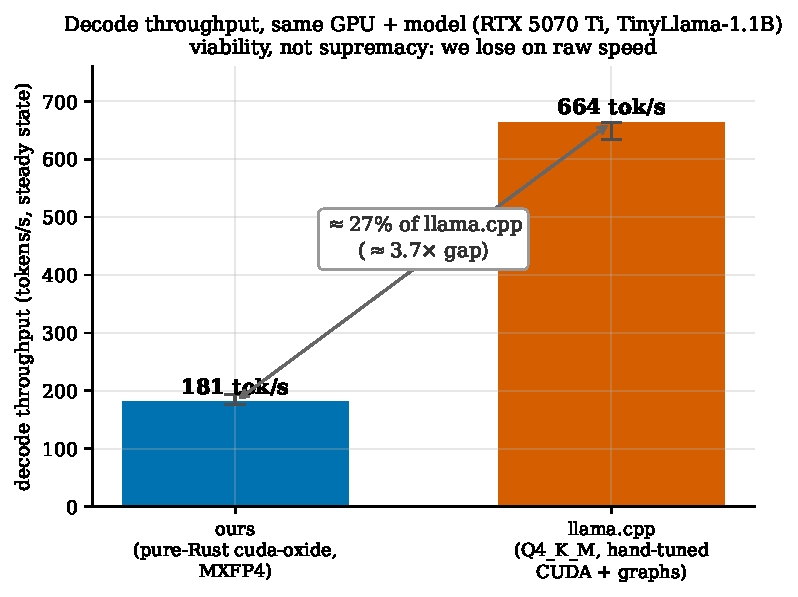
\includegraphics[width=0.78\linewidth]{figs/fig_throughput.pdf}
\caption{Decode head-to-head, steady-state on an uncontended GPU (TinyLlama-1.1B, 4-bit, RTX 5070 Ti): ours $\approx 181$\,tok/s (median; 188.6 original session) versus \texttt{llama.cpp} $\approx 664$ (634--664; 633.9 original)---about 27\% of its decode throughput, a $\approx 3.7\times$ gap. The honest result on a first, unoptimized cut; we make no supremacy claim.}
\label{fig:h2h}
\end{figure}

\textbf{Fairness caveats, stated explicitly.} The comparison is close but not apples-to-apples. Quantization differs: ours is MXFP4 (E2M1, per-32 power-of-two scale), theirs is Q4\_K\_M, a different 4-bit scheme, and we have not normalized for any quality or layout difference. The measurement harness differs: our figure is short-context decode, theirs is \texttt{llama-bench}'s tg128; we report decode throughput on both, but the exact harness differs. And we have no prefill path: \texttt{llama.cpp} prefill (pp512) reaches $\sim$30--33k\,tok/s using tensor cores, while we measure decode only --- that is our chosen lane, and it means we do not compete on prefill at all. We make \textbf{no supremacy claim}. We lose on raw speed today; the point of the comparison is the magnitude of the gap on a first attempt, which the next section accounts for.

\section{Limitations}
The $\approx\!3.7\times$ gap is explained by specific, addressable engineering, not by the language or the compiler. The engine issues roughly 200 unfused kernel launches per token, where \texttt{llama.cpp} uses CUDA graphs to drive launch overhead to near zero --- kernel fusion and/or CUDA graphs are the single largest expected win. Our FP4 GEMV runs at 30--41\% of the 896\,GB/s ceiling, where a tuned engine runs near peak; vectorized shared-memory loads, async-copy pipelining, and multi-row-per-warp scheduling are the levers. We use f32 activations, where \texttt{llama.cpp} uses f16, halving activation traffic and enabling faster math. Adding a compute-bound prefill path would broaden the comparison, though prefill is the regime where consumer Blackwell loses the datacenter speed-of-light GEMM, so we expect it to be the weaker lane and have not chased it. We have not isolated each lever's contribution to the $\approx\!3.7\times$: we order them by expected impact from the measured behavior --- the roughly 200 unfused launches per token, the GEMV's 30--41\% fraction of the bandwidth ceiling, and the f32 activation width --- not from a per-lever ablation we did not run. The three are also independent, so the wins are expected to compound rather than overlap.

The honest standing edges: the engine is decode-only and bandwidth-bound by design; the datacenter speed-of-light GEMM path is simply unavailable on consumer Blackwell; we measured a single GPU and SKU; and \texttt{cuda-oxide} is alpha and pre-1.0, so these results are a snapshot of a moving toolchain. The novelty claim of \S\ref{sec:fp4} is hedged: as far as we found, the FP4 MMA is a first, but we did not search prior art exhaustively. We exclude one earlier low reading (a 156\,tok/s figure) from the results entirely; it was a measurement artifact from timing only 48 generated tokens during the GPU's post-idle clock-ramp, fixed by timing 200 tokens at steady state, and we note it only as a methodology lesson. None of these edges is a dead end --- the runway above is concrete and ordered by expected impact.

\section{Conclusion}
We did not set out to beat \texttt{llama.cpp}, and we did not. We set out to find whether NVIDIA's own experimental Rust$\rightarrow$PTX backend can compile a real, FP4-quantized LLM decoder, written entirely in pure Rust, into kernels that run on a consumer GPU and generate coherent text --- and it can. Along the way we measured the actual Rust-programmable surface of consumer Blackwell and found it richer than the secondary sources said: TMA, clusters with distributed shared memory, and native FP4 block-scaled tensor-core MMA all execute, while the \texttt{tcgen05} datacenter pipeline correctly does not. The first cut lands within about $3.7\times$ of the hand-tuned \texttt{llama.cpp} baseline on the same hardware and model, and the gap is accounted for by ordinary, ordered optimization work --- kernel fusion, GEMV tuning, f16 activations --- not by anything fundamental to Rust or the compiler. The substrate is real, and the path is end to end. That is the result: viability, measured, with the edges named.

\appendix
\section{Reproducibility}
\label{sec:repro}
\textbf{Hardware.} RTX 5070 Ti (GB203, \texttt{sm\_120}, compute capability 12.0), driver 596.49, under WSL2 Ubuntu 24.04. \textbf{Toolchain.} \texttt{cuda-oxide} v0.2.1 (built from source, commit \texttt{7dbd192}), Rust \texttt{nightly-2026-04-03}, bundled LLVM 22.1.2 and clang-21. The FP4 block-scaled MMA requires building with \texttt{--arch sm\_120a}; plain \texttt{sm\_120} rejects the instruction. \textbf{CUDA toolkits --- note the split.} The \texttt{cuda-oxide} PTX path used the machine's CUDA 13.1 \texttt{ptxas} (which supports \texttt{sm\_120a}); the \texttt{llama.cpp} baseline was built against CUDA 12.9, because the 13.1 install lacks cuBLAS while 12.9 is the full toolkit (its \texttt{ptxas} also supports \texttt{sm\_120a}). These are two different uses of two different toolkits; we do not conflate them. \textbf{Measurement conditions.} Decode throughput is measured at steady state on an uncontended GPU: the box has two cards and host-side processes may share one, so we pinned both engines to the idle card and timed 200 tokens to clear the post-idle clock-ramp; each generation follows a $\sim$22\,s host-bound model load, so short timing windows read our engine low. No clock throttling was observed. We only compare engines measured back-to-back in the same session.

\bibliographystyle{plainnat}
\bibliography{\jobname}
\end{document}
